\documentclass[12pt,a4paper]{article}

\usepackage[margin=1in]{geometry}
\usepackage{graphicx}
\usepackage{booktabs}
\usepackage{array}
\usepackage{longtable}
\usepackage{caption}
\usepackage{subcaption}
\usepackage{amsmath}
\usepackage{amssymb}
\usepackage{hyperref}
\usepackage{natbib}
\usepackage{setspace}
\usepackage{float}
\usepackage{xcolor}

\hypersetup{
    colorlinks=true,
    linkcolor=black,
    citecolor=black,
    urlcolor=blue
}

\onehalfspacing

\title{\textbf{NIFTY-Sentinel: An Explainable Machine Learning Framework for Early Warning of Indian Equity Market Stress}}
\author{Deepankar Gupta \quad Dr. Mayura Tapkire\\
Department of Computer Science and Engineering (AI \& ML),\\
The National Institute of Engineering, Mysuru, India}
\date{\today}

\begin{document}

\maketitle

\begin{abstract}
Financial stress monitoring is a practical problem for market participants, risk managers, and policy observers because stress episodes usually emerge through several interacting channels rather than through price movement alone. This paper presents \textit{NIFTY-Sentinel}, an explainable machine learning framework designed to estimate the probability of elevated Indian equity market stress. The system does not attempt to predict exact NIFTY 50 prices. Instead, it frames the task as a forward-looking classification problem: given information available up to a trading date, estimate whether a stress condition is likely over a short future horizon. The framework combines market state indicators, volatility, drawdown, risk-appetite proxies, cross-asset connectedness, and latent regime estimates. It then applies time-series-aware supervised learning, ablation analysis, and model explanation to produce a dashboard-ready stress probability, warning level, regime label, and driver summary.

The project uses actual historical public-market data for NIFTY 50, India VIX, USD/INR, gold, Brent crude, S\&P 500, and US VIX, covering 4,105 observations through 18 September 2026. In walk-forward validation, the Random Forest prototype achieves mean PR AUC of 0.422, while the Logistic Regression benchmark achieves mean PR AUC of 0.400. Ablation results suggest that adding risk-appetite and connectedness layers improves the market-only baseline, although the observed gains remain modest and must be revalidated with official NSE and RBI data before final academic claims are made. The final output is deployed as both a Streamlit dashboard and a static GitHub Pages dashboard. The contribution of the project is a transparent end-to-end research pipeline for stress monitoring, not a trading signal or causal model.
\end{abstract}

\textbf{Keywords:} financial stress, NIFTY 50, explainable machine learning, regime detection, Random Forest, Hidden Markov Model, SHAP, connectedness, risk dashboard

\section{Introduction}

Financial markets frequently enter unstable states before a full crisis becomes obvious in headline index levels. In such periods, returns become more volatile, drawdowns deepen, cross-asset correlations rise, currency pressure can increase, and investor risk appetite can deteriorate. A monitoring system that uses only the level of the NIFTY 50 index may therefore miss important warning signs. The motivation behind NIFTY-Sentinel is to combine several market stress layers into one interpretable early-warning framework.

The project is designed around one main research question:

\begin{quote}
Can an explainable machine learning system provide a useful early-warning estimate of Indian equity market stress by combining market state, risk appetite, volatility, connectedness, and regime information?
\end{quote}

This question is deliberately different from the common task of index price prediction. The objective is not to forecast whether the NIFTY 50 will close at a specific level tomorrow. Instead, the objective is to estimate the probability that future market conditions will be stressful. This framing is more appropriate for decision support because risk managers and students of financial instability usually need a graded warning signal rather than a single point forecast.

The implemented system follows the initial project design: data collection, feature engineering, exploratory analysis, latent regime modelling, connectedness estimation, supervised stress classification, ablation analysis, explainability, and dashboard deployment. The system produces three user-facing outputs:

\begin{enumerate}
    \item a continuous stress probability;
    \item a discrete warning level, classified as Normal, Elevated, or Severe;
    \item an explanation layer showing regimes, feature importance, and visual evidence.
\end{enumerate}

\section{Research Objectives}

The project has five objectives.

\begin{enumerate}
    \item Construct a reproducible data pipeline for Indian market stress monitoring.
    \item Engineer interpretable stress indicators from price, volatility, currency, commodity, and global risk proxies.
    \item Detect latent market regimes using unsupervised time-series methods.
    \item Train and validate supervised models using walk-forward evaluation rather than random train-test splitting.
    \item Present the output through a dashboard that emphasizes interpretation and visual diagnosis.
\end{enumerate}

These objectives shape the full research design. The resulting paper therefore evaluates not only prediction metrics, but also whether the system is transparent enough to support disciplined interpretation.

\section{Related Work}

This project is positioned at the intersection of financial stress measurement, Indian equity-market volatility, connectedness analysis, regime detection, and explainable machine learning. The literature from 2020 onward is especially relevant because it covers the COVID-19 shock, the post-pandemic inflation and rate-tightening period, and the increasing use of interpretable machine learning in financial early-warning systems.

\subsection{Financial Stress Measurement and Early-Warning Systems}

Recent research continues to treat financial stress as a multidimensional condition rather than a single-market event. For India, \citet{sahoo2021indiafsi} constructs a financial stress index using money market, bond market, equity market, foreign exchange market, and banking-sector variables, showing that a composite view is more informative than one isolated indicator. Similarly, \citet{jfep2020indiafsi} evaluates alternative Indian financial stress indicators and finds that stress indices based on time-varying correlation methods, especially DCC-GARCH, are useful for tracing known stress periods and business-cycle weakness. These studies support the central design choice in NIFTY-Sentinel: market stress should be measured through several channels, including equity returns, volatility, currency pressure, and cross-market co-movement.

The broader early-warning literature also emphasizes realistic validation. \citet{samitas2020ml} show that combining financial networks with machine learning can improve crisis-warning performance, while \citet{duprey2022early} caution that pseudo-real-time identification of leading indicators is difficult and that apparently useful signals can become clear only after a crisis has already occurred. \citet{jarmulska2022rf} compares random forests and logit models for fiscal-stress warning and shows that machine learning can be useful, but must be evaluated against transparent benchmarks. \citet{genberg2022banking} use AdaBoost to rank determinants of banking crises across countries, while \citet{tang2024systemic} combine stress indices, Markov regime switching, and interpretable machine learning for systemic-risk prediction. Together, these papers justify the project's use of both a logistic-regression benchmark and a nonlinear random-forest model, with walk-forward validation rather than random train-test splitting.

\subsection{Indian Market Volatility, COVID-19, and Connectedness}

The Indian market literature after 2020 strongly supports the inclusion of volatility and connectedness features. \citet{guru2021covid} examine ten BSE sector indices and find that COVID-19 substantially increased sectoral volatility spillovers in India. \citet{rao2021vulnerability} study NIFTY 50 firms during India's lockdown and post-lockdown phases, documenting the market's vulnerability to pandemic information and investor sentiment. \citet{sahoo2023sectoral} find strong short-run and long-run volatility persistence among Indian sectoral indices during the COVID-19 period, with high time-varying correlations that reduce diversification benefits. \citet{eap2023indiaCommodity} extend the connectedness view to Indian equity and commodity markets, finding that volatility spillovers between Indian equities and major commodities rose after the COVID-19 outbreak. \citet{jrfm2024indiaSpillover} further show that pandemic-era volatility changed spillover patterns between India and major global markets.

These Indian-market findings are consistent with global connectedness studies. \citet{li2021asymmetric} report crisis-sensitive and asymmetric volatility spillovers across major global stock markets, with emerging markets often receiving downside risk during the 2020 crash. \citet{zhang2021oilstock} show that COVID-19 changed return and volatility spillovers between oil and stock markets. \citet{adekoya2021covidconnected} use TVP-VAR and causality-in-quantiles methods to show that pandemic uncertainty drove connectedness across commodity and financial markets. \citet{naeem2021covid} and \citet{sectoral2022us} also document a sharp rise in connectedness during the pandemic. The implication for NIFTY-Sentinel is direct: a rolling connectedness layer is theoretically and empirically justified because stress periods are often marked by stronger cross-asset co-movement.

\subsection{Volatility, Market Fear, and Risk-Appetite Proxies}

NIFTY-Sentinel uses India VIX, USD/INR, gold, crude oil, S\&P 500, and US VIX as risk-appetite and global-risk proxies. This choice is consistent with recent work on market fear and cross-asset stress transmission. \citet{marketfear2021india} study India VIX and historical NIFTY volatility during COVID-19 using machine learning, deep learning, feature selection, and explainable AI, and show that market fear measures can be predicted from macroeconomic, technical, and search-based features. \citet{panga2021oilfsi} connect financial stress to oil-market realized volatility through Markov-regime-switching MIDAS models, which supports the inclusion of commodity variables in stress-monitoring frameworks. \citet{zhang2021oilstock} and \citet{eap2023indiaCommodity} similarly show that crude oil and commodity markets can become important channels of equity-market volatility transmission.

This literature suggests that stress-monitoring models should not rely only on domestic index returns. Risk appetite often deteriorates through implied volatility, exchange-rate pressure, safe-haven demand, commodity shocks, and global equity-market volatility. The project's feature layers therefore follow a defensible empirical pattern: price, volatility, currency, commodity, global risk, connectedness, and regime information are treated as complementary rather than competing inputs.

\subsection{Regime Detection and Explainable Machine Learning}

Recent studies also support the use of latent regimes and explanation tools. \citet{giudici2020hmm} apply Hidden Markov Models to detect bull, stable, and bear regimes in cryptoasset markets, illustrating the usefulness of unobserved-state models for volatile financial series. \citet{dua2021regime} use Markov-switching models to study regime shifts and dynamic linkages across currency and equity markets, including India. \citet{fons2020hmm} develop a dynamic asset-allocation system using feature-saliency Hidden Markov Models, showing that regime identification can be strengthened by feature selection. These papers support the project's use of an HMM regime feature, while also motivating caution: regime labels should be interpreted as compact statistical summaries, not as causal explanations.

The explainable-AI literature is equally relevant. \citet{zhang2022xai} propose an explainable AI framework for financial distress prediction using Shapley additive explanations, partial dependence plots, and counterfactual explanations. \citet{tang2024systemic} use interpretable machine learning to identify influential systemic-risk indicators, and \citet{asoc2023xai} review how explainability can extend financial time-series prediction models. \citet{survey2022fts} survey machine-learning models for financial time-series forecasting and highlight the difficulty of nonlinear, dynamic, and noisy financial data. These findings support the project's decision to report feature importance and SHAP-style explanations alongside performance metrics. For a financial stress dashboard, interpretability is not decorative; it is necessary for users to judge whether a warning is economically plausible.

The same decision-support perspective appears in applied AI studies outside finance. Recent work has used machine learning for food and disease-risk analysis, road navigation, facial emotion and expression recognition, cardiac screening, gluten identification, skin-lesion analysis, diabetes detection, plant-disease detection, remote health monitoring, and cognitive-impairment assessment \citep{tapkire2023food,arun2024road,lavanya2024emotion,shashidhar2025heart,tapkire2025gluten,manjunath2025skin,natesh2025diabetes,lavanya2024facialreview,shwetha2026plant,arpitha2025health,vinesh2026mci,lavanya2026mcipred}. Although these applications do not provide direct evidence about financial stress, they illustrate a common requirement across applied machine-learning systems: model outputs become more useful when they are validated, interpretable, and presented with the limits of the underlying evidence.

\subsection{Research Gap Addressed by NIFTY-Sentinel}

The reviewed literature establishes four facts. First, Indian financial stress is better represented by composite, cross-market indicators than by equity prices alone. Second, COVID-19 and later global shocks increased volatility spillovers and connectedness, especially across equities, commodities, currencies, and global risk proxies. Third, machine-learning early-warning systems can be useful, but their apparent performance must be tested with time-aware validation and transparent benchmarks. Fourth, explainability and regime diagnosis are essential when model outputs are used for financial monitoring.

NIFTY-Sentinel responds to this gap by combining these ideas in one reproducible pipeline for Indian equity-market stress. It does not claim to forecast exact NIFTY 50 prices. Instead, it estimates a forward-looking probability of elevated stress using market-state features, volatility, drawdown, risk-appetite proxies, rolling connectedness, HMM regimes, walk-forward supervised learning, ablation analysis, and explainability outputs. This integrated design is the project's main contribution relative to the recent literature.

\section{Data}

\subsection{Prototype Data Sources}

The current implementation uses actual historical public-market data downloaded through a market-data interface and committed with the repository. The prototype includes:

\begin{itemize}
    \item NIFTY 50 close;
    \item India VIX;
    \item USD/INR exchange rate;
    \item gold futures;
    \item Brent crude oil;
    \item S\&P 500;
    \item US VIX.
\end{itemize}

The local dataset contains 4,105 aligned observations and currently runs through 18 September 2026. These are real historical market observations from public symbols and are used throughout the pipeline and dashboard. For a final academic submission, the public-market inputs should be verified against official NSE and RBI sources where possible. The project repository includes a separate official-data import path for files such as \texttt{nifty50\_nse.csv}, \texttt{india\_vix\_nse.csv}, \texttt{nifty\_bank\_nse.csv}, and \texttt{gsec\_10y\_rbi.csv}.

\subsection{Data Governance and Limitations}

The distinction between public-market data and official exchange or central-bank archives is important. The figures and metrics in this paper are computed from actual historical public-market data. They should not be interpreted as official NSE/RBI-verified findings until the official data path is populated and the notebooks are rerun. This limitation is not a weakness of the design; it is a necessary safeguard against unsupported financial claims.

\section{Feature Engineering}

The feature set is organized into four conceptual layers. Table~\ref{tab:feature_layers} summarizes the design.

\begin{table}[H]
\centering
\caption{Feature layers used in NIFTY-Sentinel}
\label{tab:feature_layers}
\begin{tabular}{p{0.23\textwidth} p{0.34\textwidth} p{0.32\textwidth}}
\toprule
\textbf{Layer} & \textbf{Examples} & \textbf{Interpretation} \\
\midrule
Market state & log return, 20-day momentum, 60-day drawdown & Measures the direction and depth of equity market movement. \\
Volatility & 5-day, 20-day, and 60-day rolling volatility & Captures short-term and medium-term instability. \\
Risk appetite & India VIX change, USD/INR return, gold return & Represents risk aversion, currency pressure, and defensive asset demand. \\
Connectedness & rolling mean absolute cross-asset correlation & Detects whether assets are moving together during stress. \\
Regime & HMM latent state & Summarizes unobserved market conditions. \\
\bottomrule
\end{tabular}
\end{table}

The stress target is constructed as a forward-looking label over a short horizon. The label is based on future adverse movement and volatility conditions, while the cutoff is estimated from historical information available before the prediction date. This design reduces look-ahead bias compared with a label that uses future information to define both the event and the threshold.

\section{Exploratory Data Analysis}

Exploratory data analysis is used to understand whether the raw market features behave consistently with known stress behavior. Figure~\ref{fig:eda_drawdown_volatility} shows the NIFTY 50 close, 60-day drawdown, and 20-day rolling volatility. The figure demonstrates why a stress system should include more than price level. The index can recover in level while drawdown and volatility still contain information about market fragility.

\begin{figure}[H]
\centering
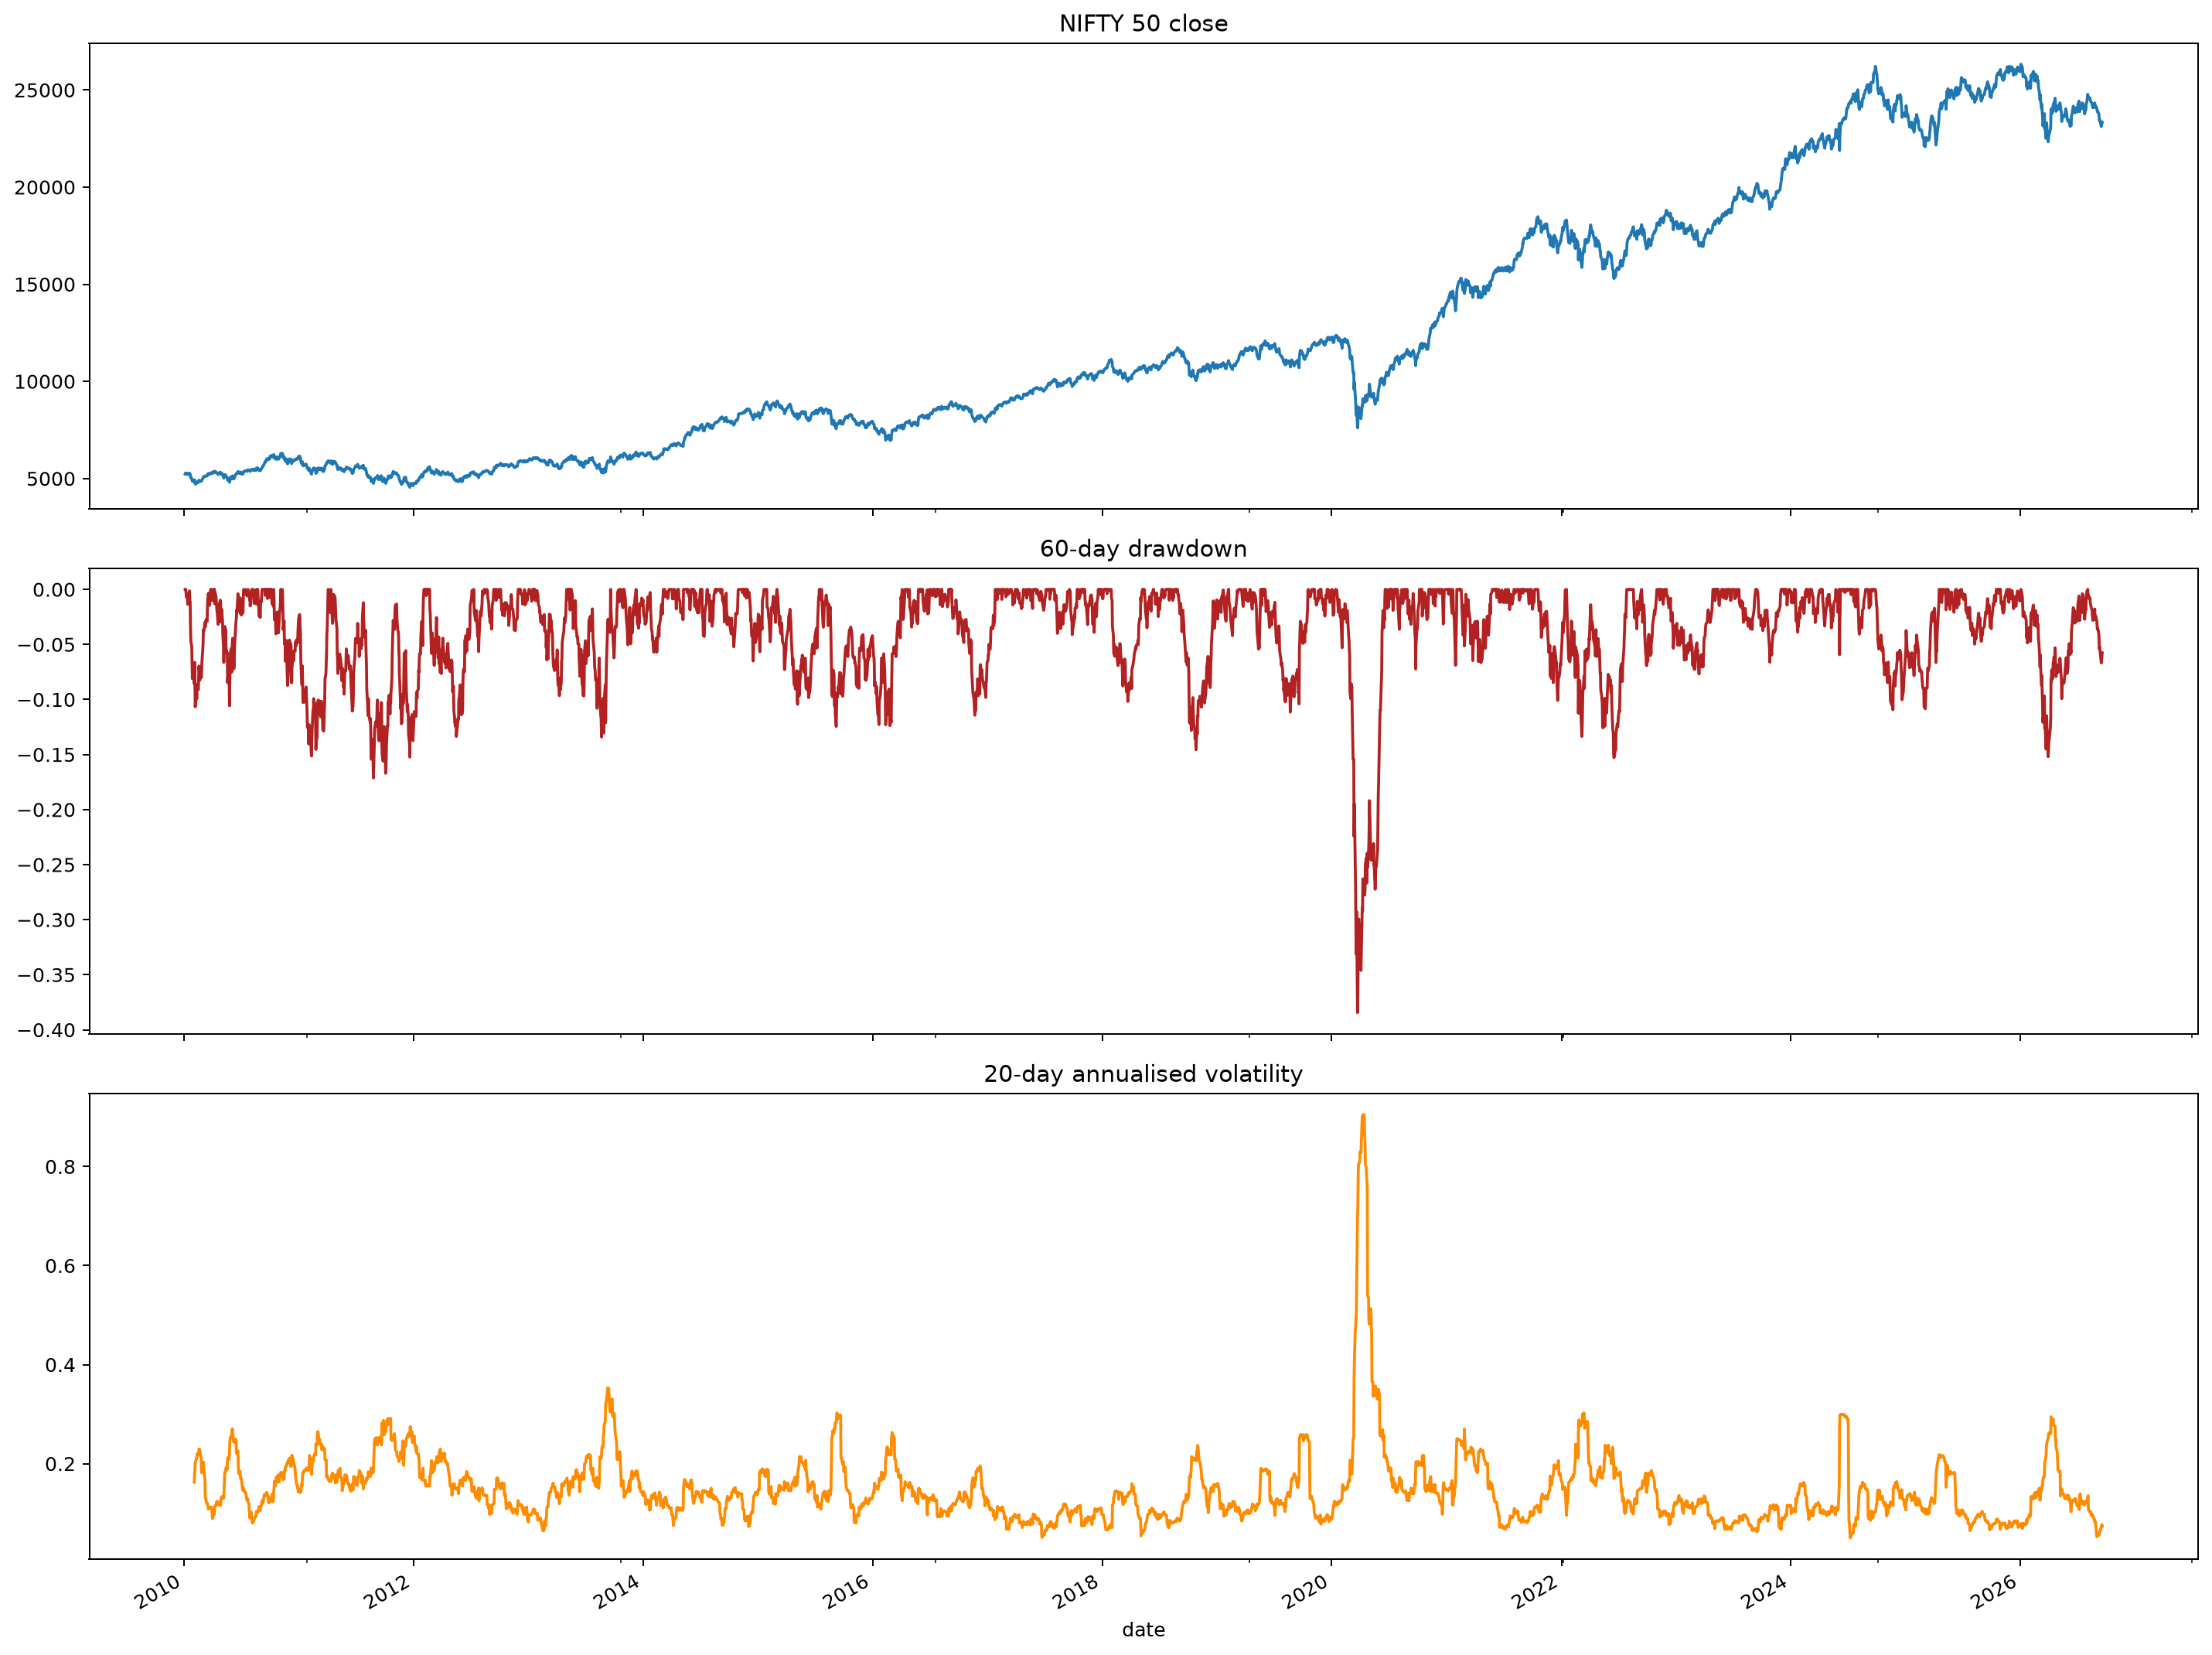
\includegraphics[width=0.95\textwidth]{figures/eda_nifty_drawdown_volatility.png}
\caption{NIFTY 50 close, drawdown, and volatility. The figure shows that stress is not only a price-level phenomenon; volatility and drawdown capture different aspects of market instability.}
\label{fig:eda_drawdown_volatility}
\end{figure}

Figure~\ref{fig:return_correlation} presents the return correlation heatmap across the selected market proxies. Correlation analysis is useful because systemic stress often appears as a rise in common movement across otherwise distinct assets. This motivates the connectedness layer used later in the modelling pipeline.

\begin{figure}[H]
\centering
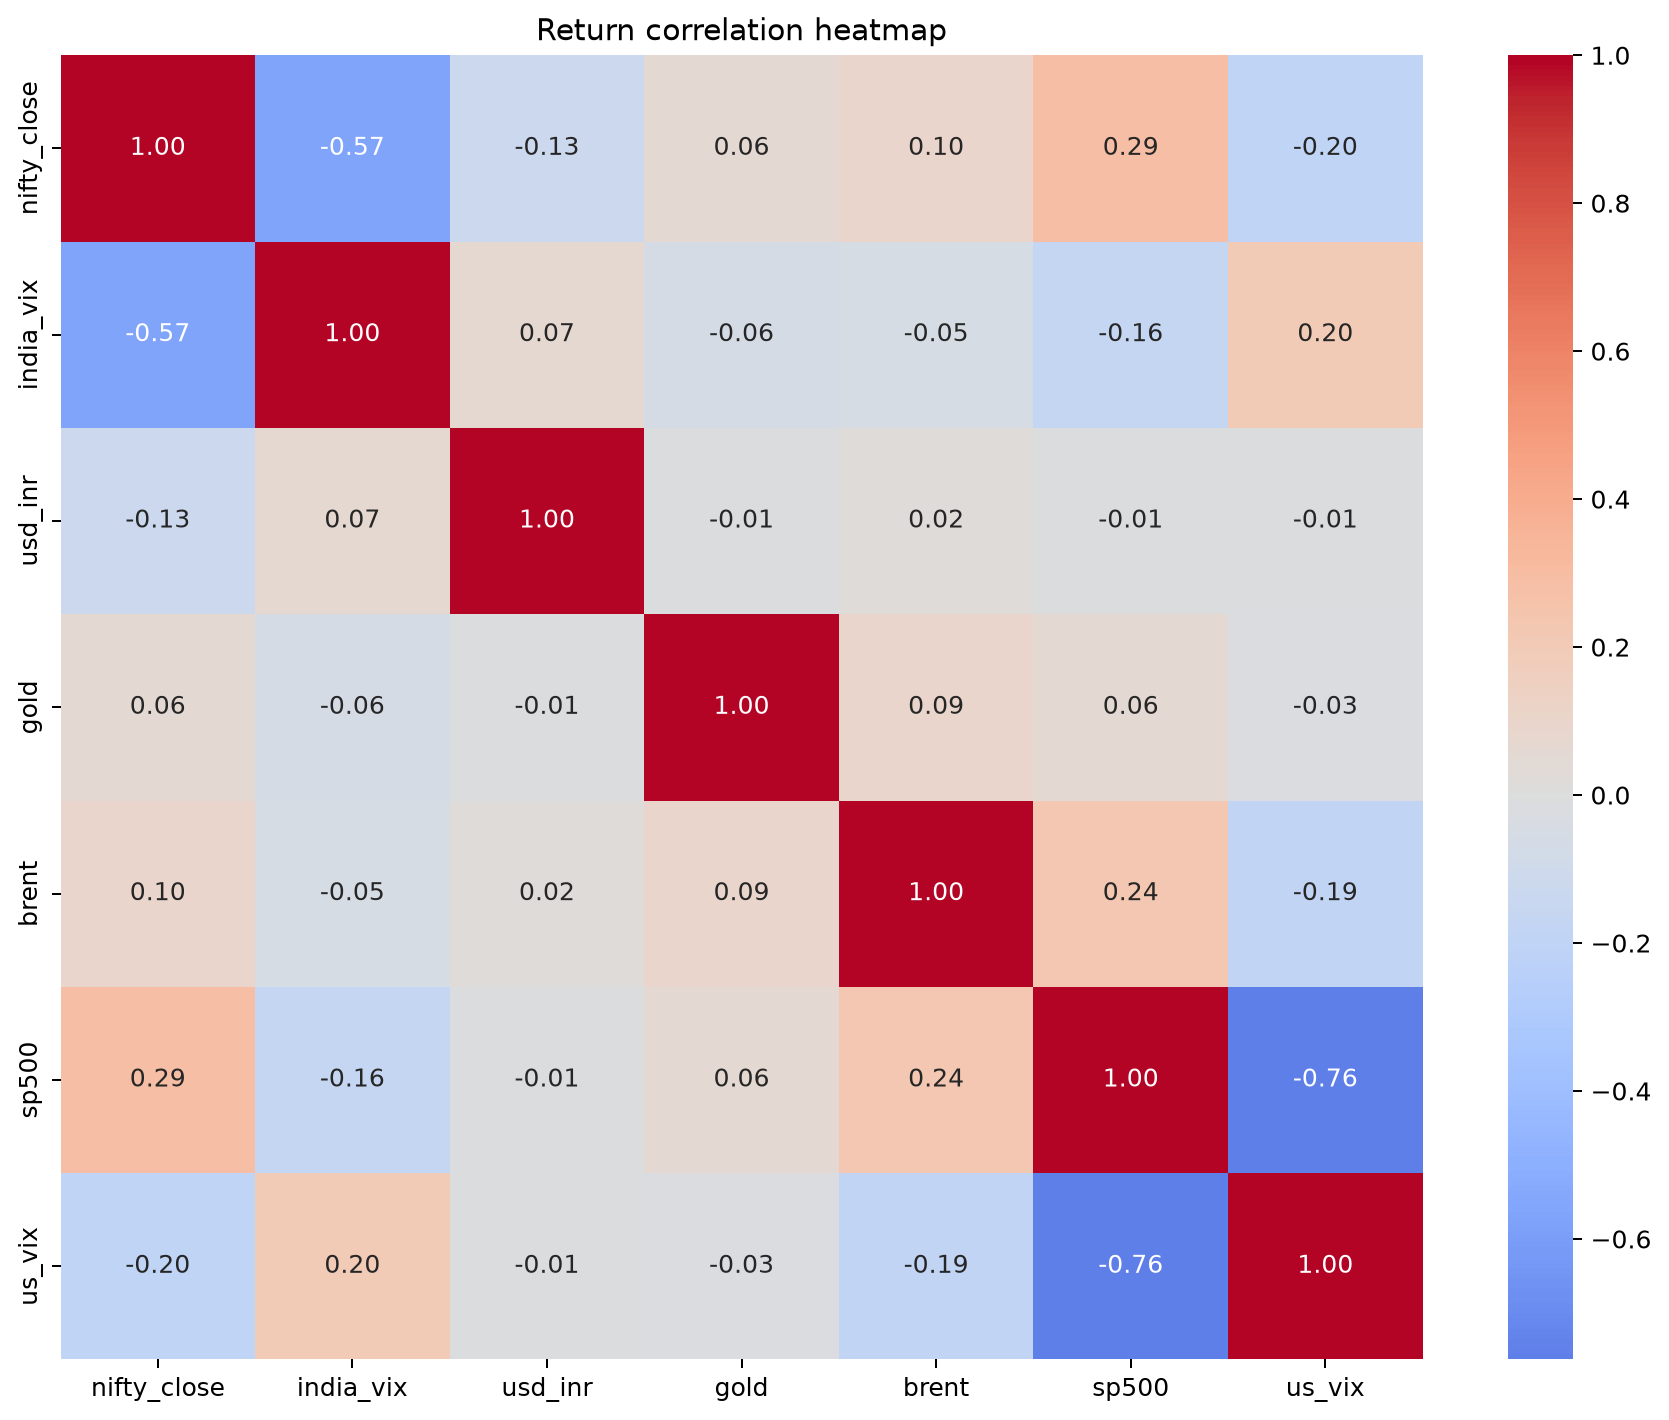
\includegraphics[width=0.78\textwidth]{figures/eda_return_correlation_heatmap.png}
\caption{Return correlation heatmap for the actual historical market variables. Stronger absolute correlations indicate channels through which market stress may propagate across assets.}
\label{fig:return_correlation}
\end{figure}

\section{Methodology}

\subsection{Regime Detection}

The project uses a Gaussian Hidden Markov Model with three latent states. The model is trained on standardized market-state features, including return, volatility, drawdown, India VIX change, and USD/INR return. The purpose of the HMM is not to create a final label by itself, but to add a regime feature that summarizes market context.

Figure~\ref{fig:hmm_regimes} plots the NIFTY 50 with inferred regimes. Visually, the regimes separate periods with different volatility and drawdown behavior. Such states are useful for the supervised model because the same return shock may have different implications depending on the prevailing regime.

\begin{figure}[H]
\centering
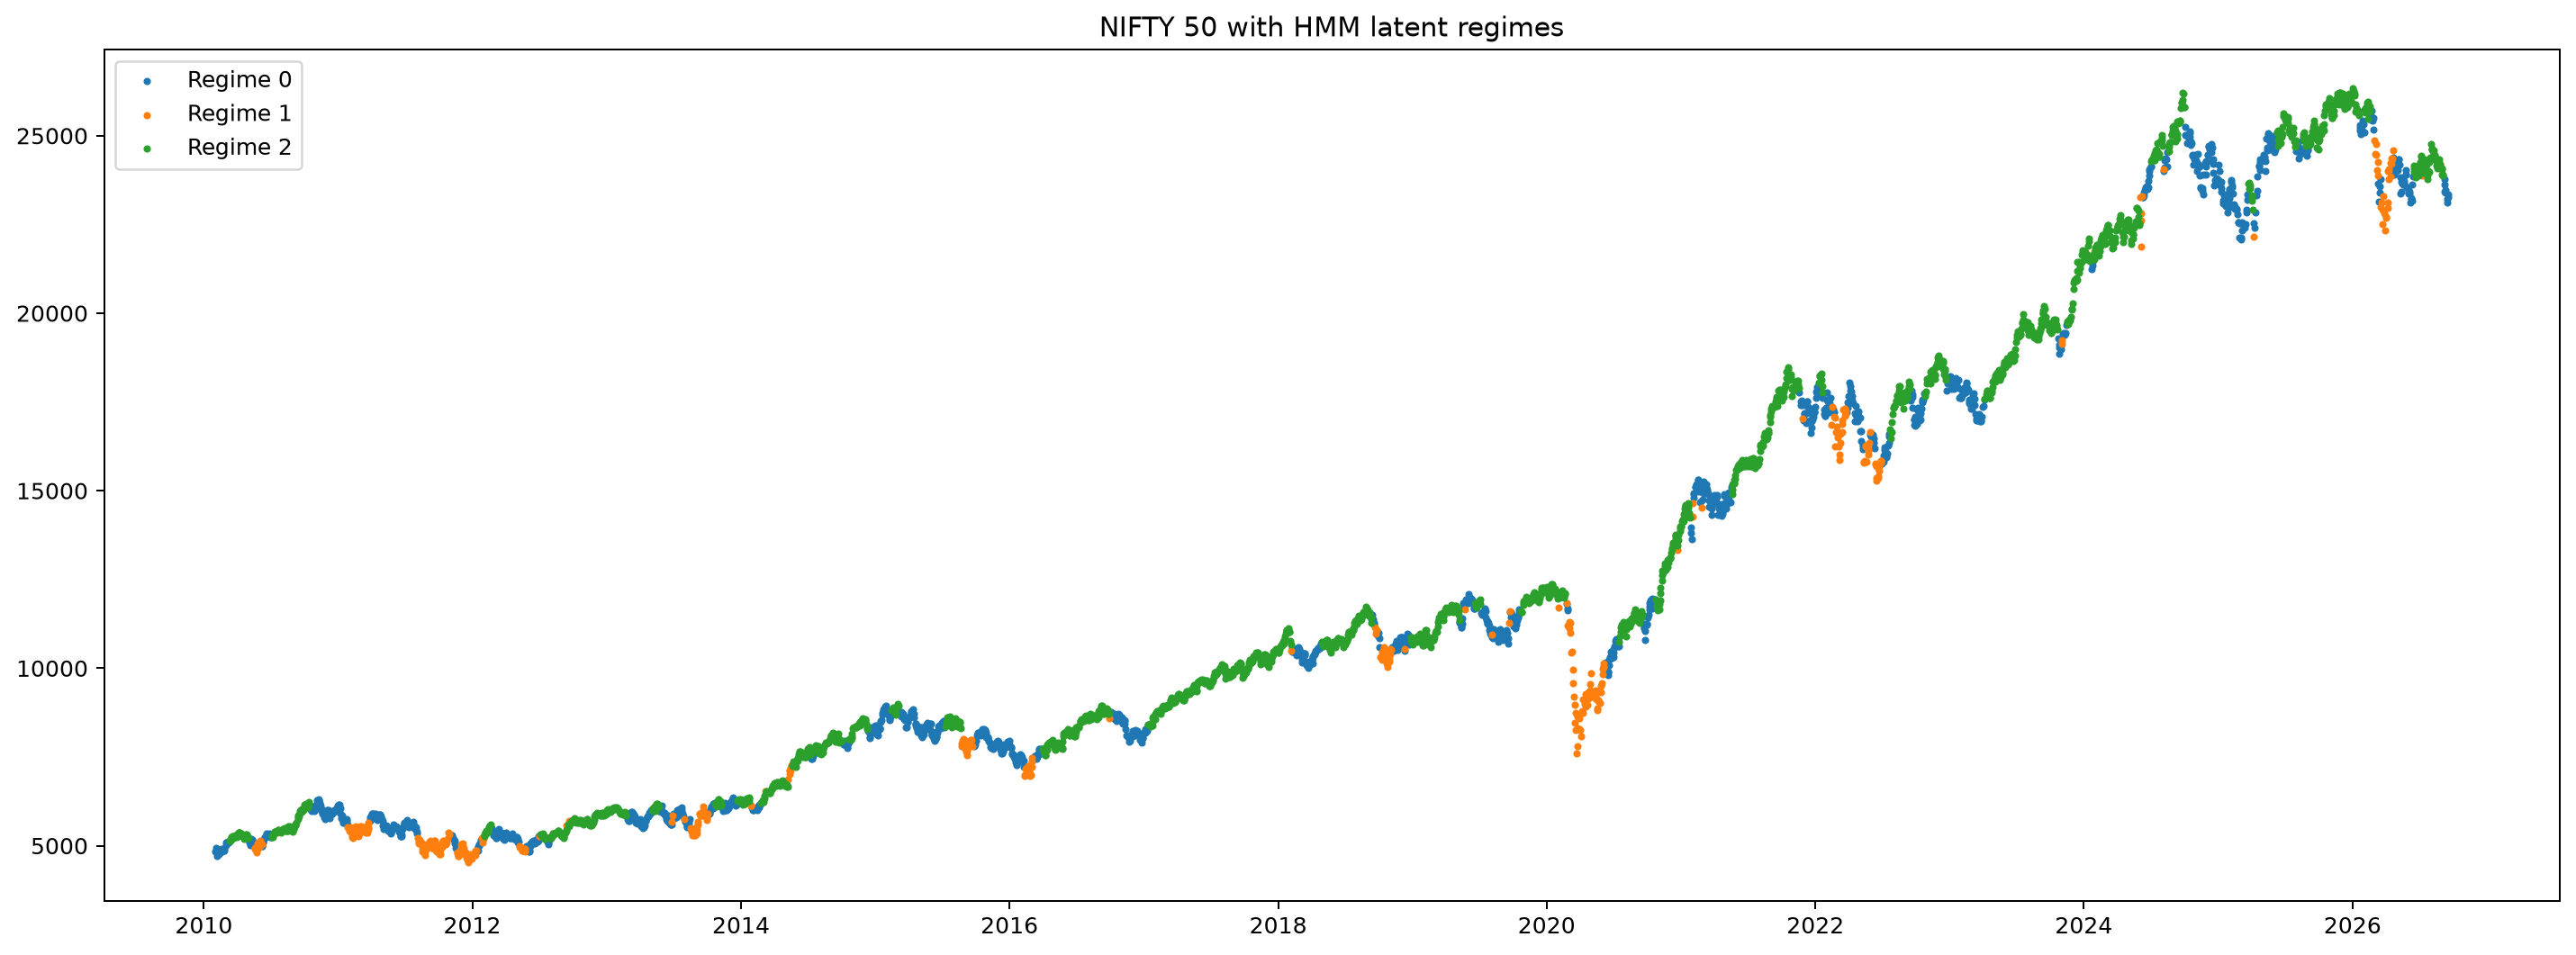
\includegraphics[width=0.95\textwidth]{figures/hmm_regimes_nifty.png}
\caption{NIFTY 50 with HMM latent regimes. The regime layer gives the supervised model a compact representation of changing market conditions.}
\label{fig:hmm_regimes}
\end{figure}

\subsection{Connectedness}

Connectedness is measured with a 60-day rolling mean absolute cross-asset correlation. The intuition is that markets often become more synchronized during stress. When correlations rise across equity, currency, commodity, and global risk proxies, diversification benefits may decline and stress can spread more easily.

Figure~\ref{fig:connectedness} shows the rolling connectedness measure. Peaks in this figure indicate periods when cross-asset co-movement became unusually strong. In the NIFTY-Sentinel dashboard, this measure is displayed alongside stress probability so that users can evaluate whether a warning is supported by broader market synchronization.

\begin{figure}[H]
\centering
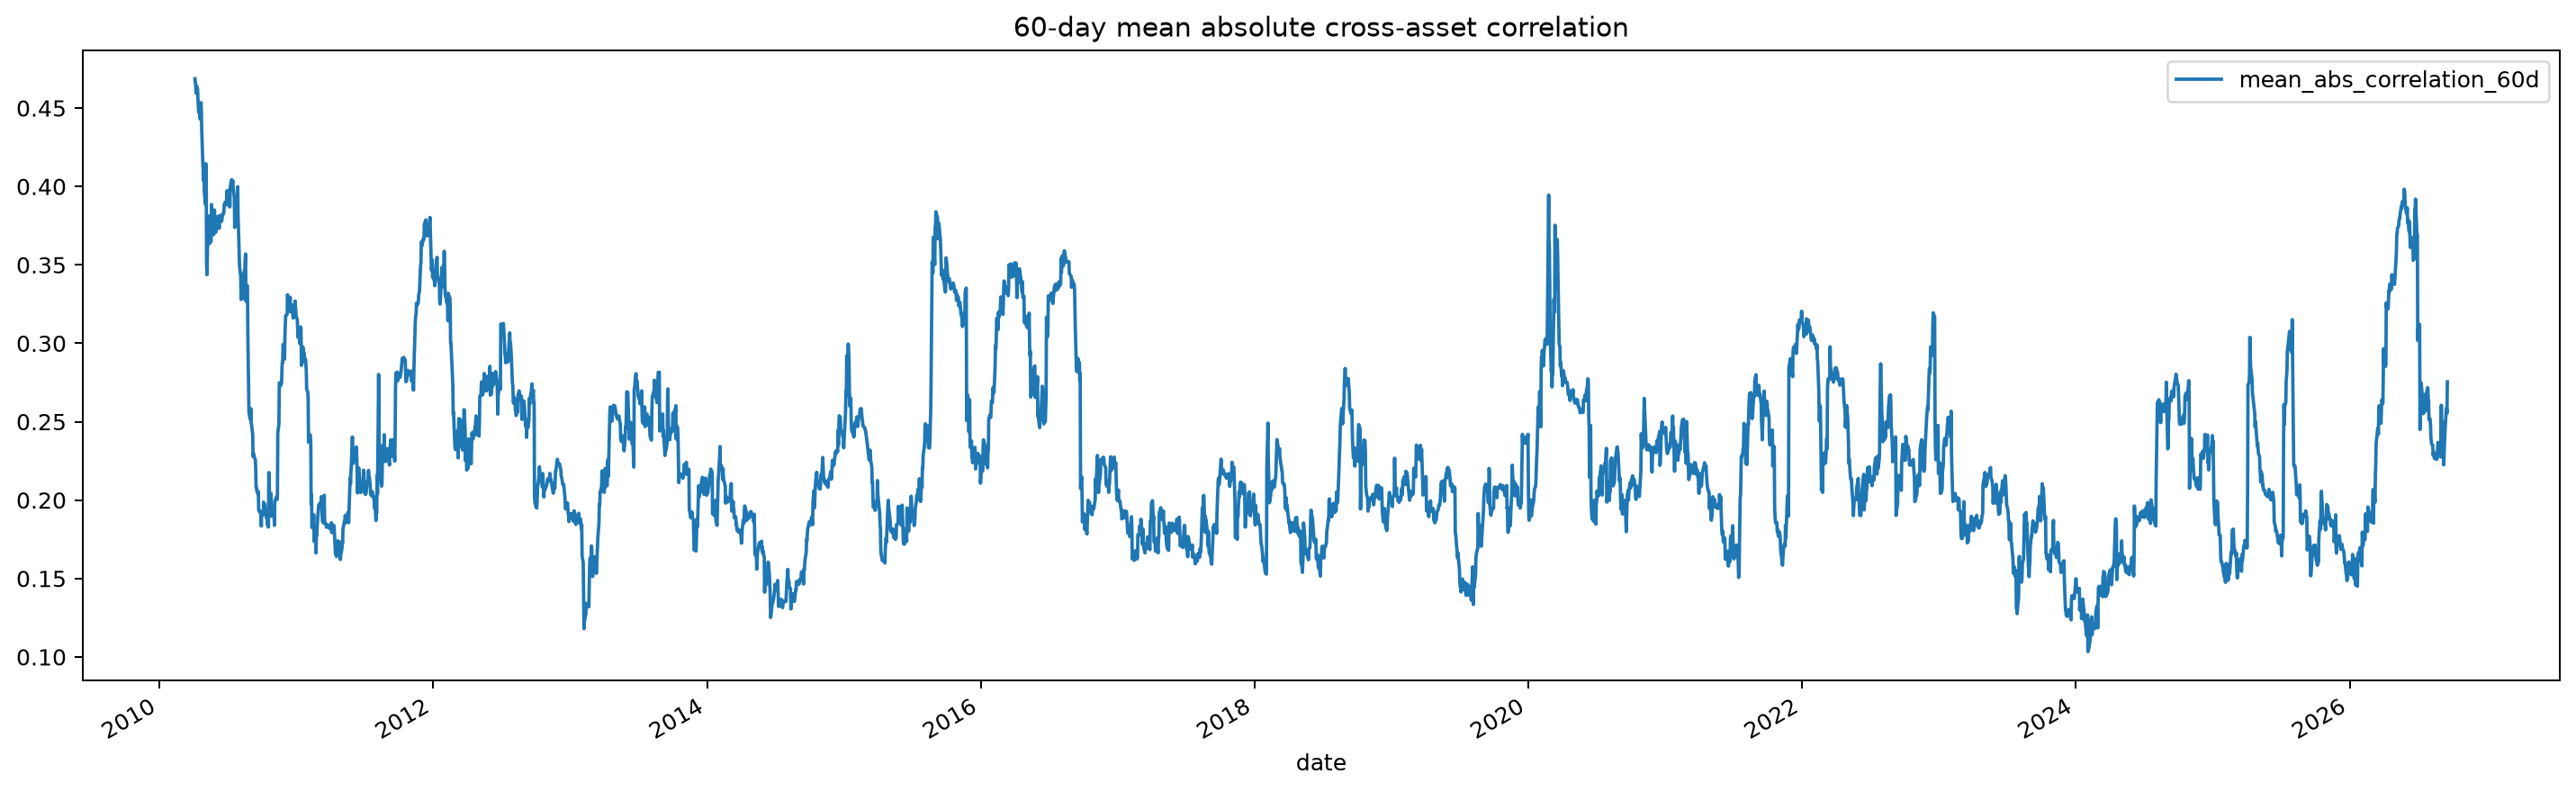
\includegraphics[width=0.95\textwidth]{figures/rolling_connectedness.png}
\caption{Rolling 60-day mean absolute cross-asset correlation. Higher values indicate stronger market-wide co-movement and potential systemic stress.}
\label{fig:connectedness}
\end{figure}

\subsection{Supervised Learning}

The supervised classification task estimates the probability of future stress. Two model families are used:

\begin{enumerate}
    \item Logistic Regression, included as a transparent linear benchmark.
    \item Random Forest, included as a nonlinear ensemble model capable of capturing interactions.
\end{enumerate}

Missing values are handled through median imputation inside modelling pipelines. The evaluation uses time-series splits. This is essential because random shuffling would allow later observations to influence earlier train-test comparisons, creating an unrealistic validation setting.

\subsection{Warning-Level Mapping}

The continuous stress probability is converted into three warning bands:

\begin{equation}
\text{Warning} =
\begin{cases}
\text{Normal}, & p < 0.30 \\
\text{Elevated}, & 0.30 \leq p < 0.60 \\
\text{Severe}, & p \geq 0.60
\end{cases}
\end{equation}

These thresholds are simple and interpretable. In a production environment, they should be calibrated against user-specific costs of false alarms and missed stress events.

\section{Results}

\subsection{Walk-Forward Model Performance}

Table~\ref{tab:model_results} reports the average walk-forward performance of the two supervised models. Random Forest has a slightly higher mean PR AUC than Logistic Regression, while ROC AUC is similar. PR AUC is especially relevant because stress events are less frequent than normal periods.

\begin{table}[H]
\centering
\caption{Mean walk-forward performance}
\label{tab:model_results}
\begin{tabular}{lcc}
\toprule
\textbf{Model} & \textbf{Mean ROC AUC} & \textbf{Mean PR AUC} \\
\midrule
Logistic Regression & 0.740 & 0.400 \\
Random Forest & 0.734 & 0.422 \\
\bottomrule
\end{tabular}
\end{table}

The result should be interpreted cautiously. The prototype shows that the nonlinear model is useful, but not overwhelmingly superior. This is common in financial stress prediction because the signal is noisy and regime-dependent. A valuable dashboard should therefore show probability and explanatory context rather than only a binary model output.

\subsection{Ablation Study}

The ablation study evaluates whether each information layer contributes to the stress classifier. Table~\ref{tab:ablation} summarizes the average results.

\begin{table}[H]
\centering
\caption{Mean ablation results by information layer}
\label{tab:ablation}
\begin{tabular}{lccc}
\toprule
\textbf{Configuration} & \textbf{PR AUC} & \textbf{Precision} & \textbf{Recall} \\
\midrule
Market baseline & 0.400 & 0.459 & 0.348 \\
Market plus risk appetite & 0.413 & 0.492 & 0.350 \\
Market plus risk and liquidity & 0.413 & 0.492 & 0.350 \\
Market plus risk and connectedness & 0.419 & 0.513 & 0.355 \\
Full NIFTY-Sentinel & 0.420 & 0.508 & 0.343 \\
\bottomrule
\end{tabular}
\end{table}

Figure~\ref{fig:ablation} visualizes the same ablation comparison. The market-only baseline is improved by adding the risk-appetite and connectedness layers. The full model has the highest PR AUC, although the improvement is modest. This supports the central design principle of the project: stress monitoring should combine several interpretable channels, but added complexity must be justified empirically.

\begin{figure}[H]
\centering
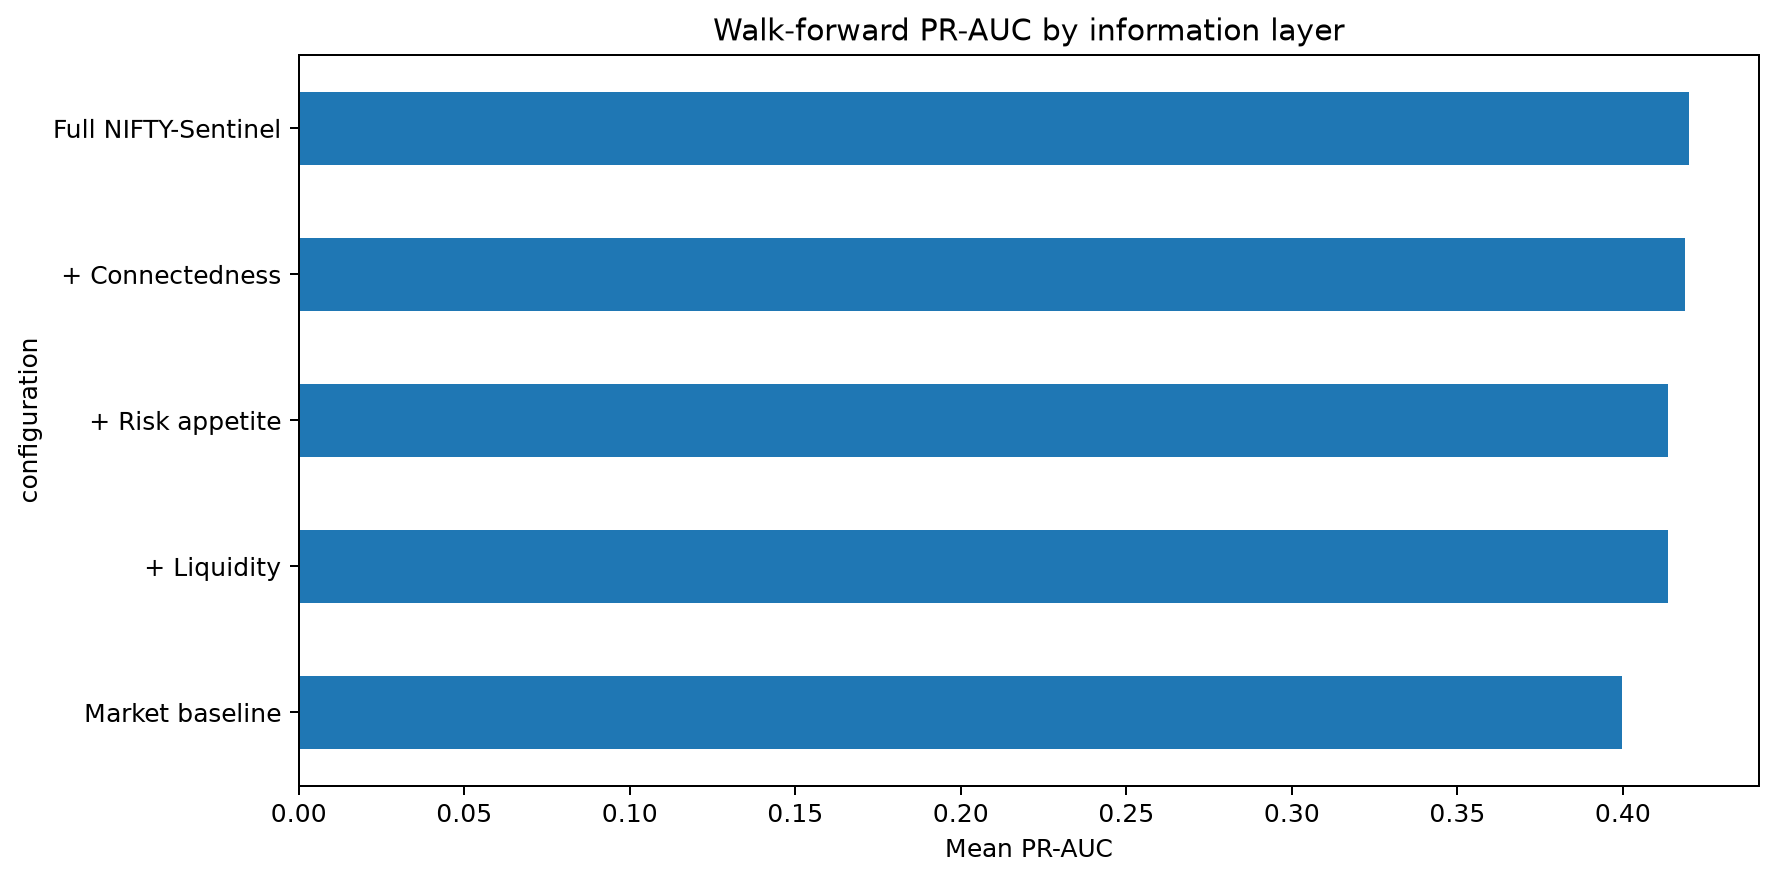
\includegraphics[width=0.82\textwidth]{figures/ablation_pr_auc.png}
\caption{Walk-forward PR AUC by information layer. The ablation study shows that risk-appetite and connectedness information improve the market baseline in the prototype.}
\label{fig:ablation}
\end{figure}

\subsection{Stress Probability Timeline}

Figure~\ref{fig:stress_timeline} shows the model's predicted stress probability over time. The plot is the core output of the system because it transforms many features into a single interpretable warning series. The horizontal thresholds map the probability into Normal, Elevated, and Severe bands.

\begin{figure}[H]
\centering
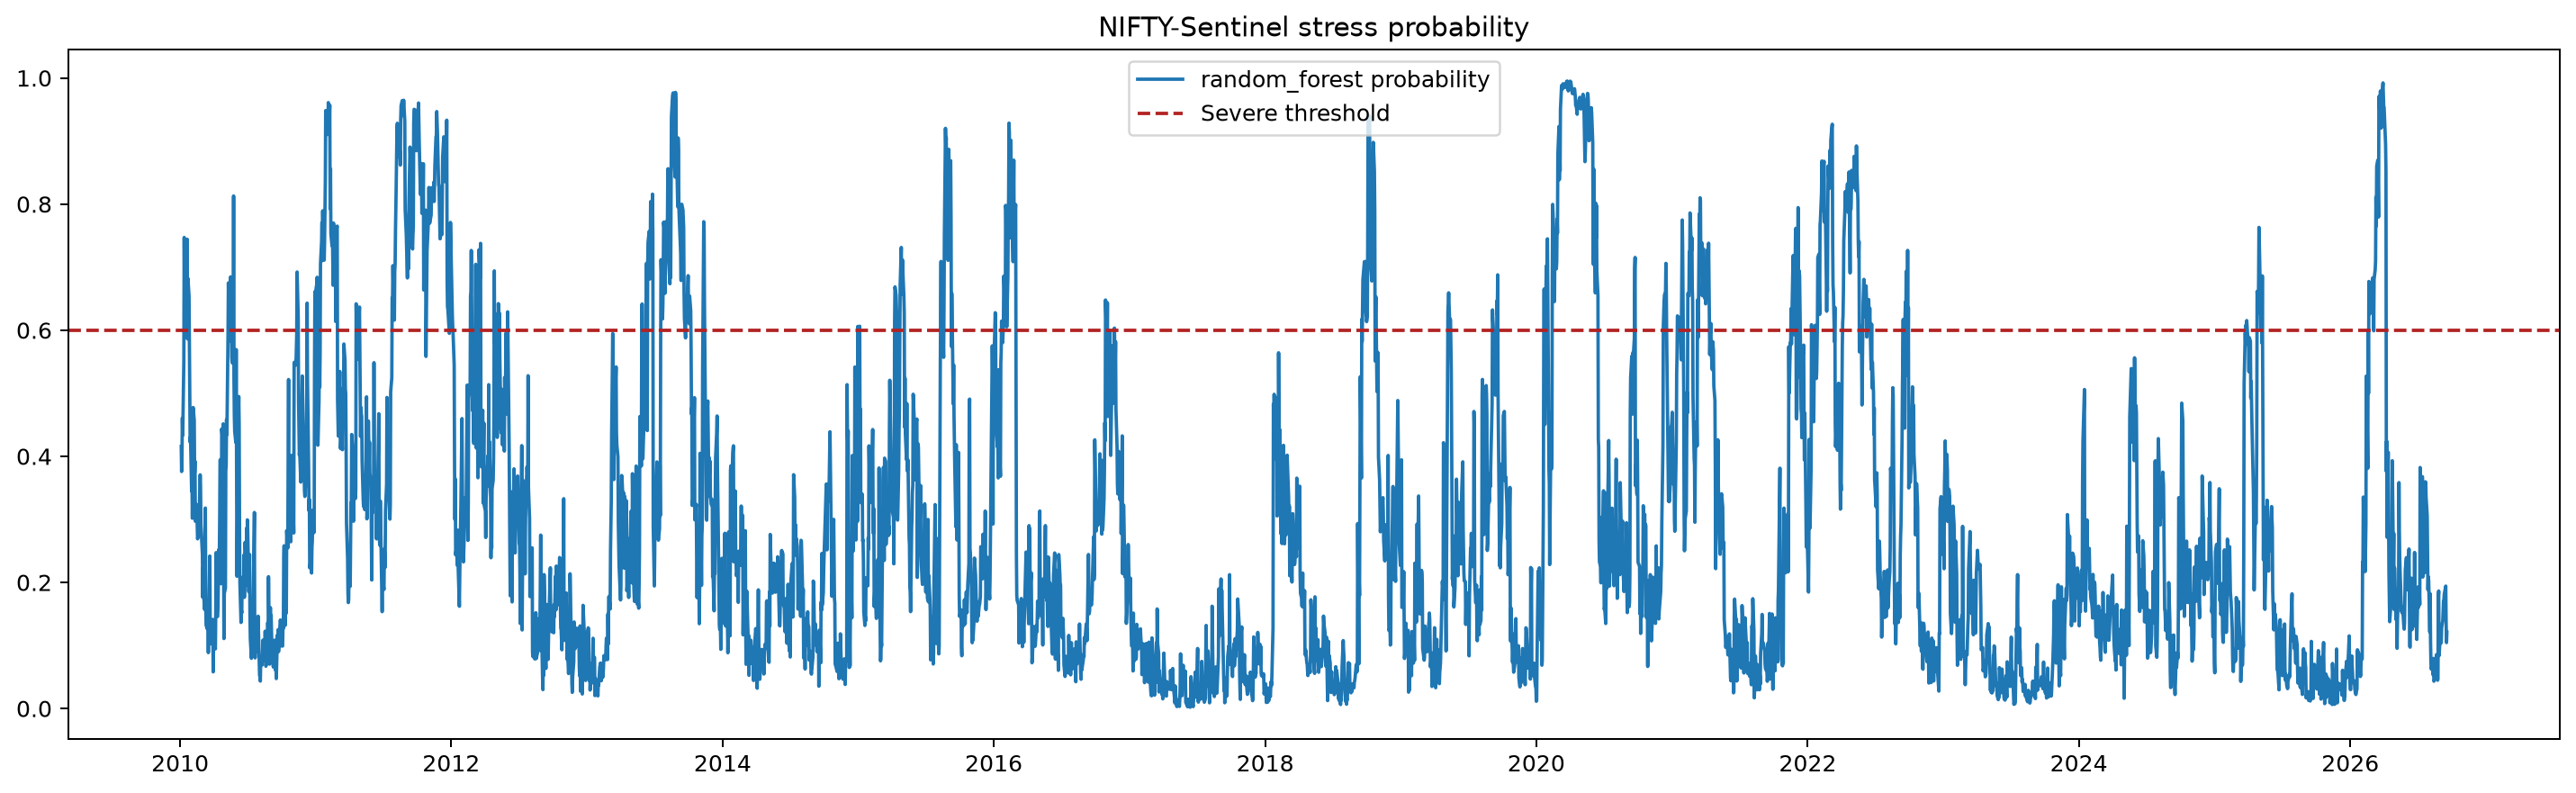
\includegraphics[width=0.95\textwidth]{figures/stress_probability_timeline.png}
\caption{Predicted market-stress probability timeline. The probability series provides the dashboard's primary early-warning signal.}
\label{fig:stress_timeline}
\end{figure}

In the latest dashboard export, the final available date is 18 September 2026. The latest stress probability is approximately 0.137, corresponding to the Normal warning band. Across the full prototype sample, the dashboard records 2,691 Normal observations, 782 Elevated observations, and 632 Severe observations.

\subsection{Explainability}

Explainability is important because a black-box warning is difficult to trust in a financial setting. The project therefore includes feature-importance and SHAP-style explanation outputs. Figure~\ref{fig:shap} shows the feature summary plot generated by the explainability notebook.

\begin{figure}[H]
\centering
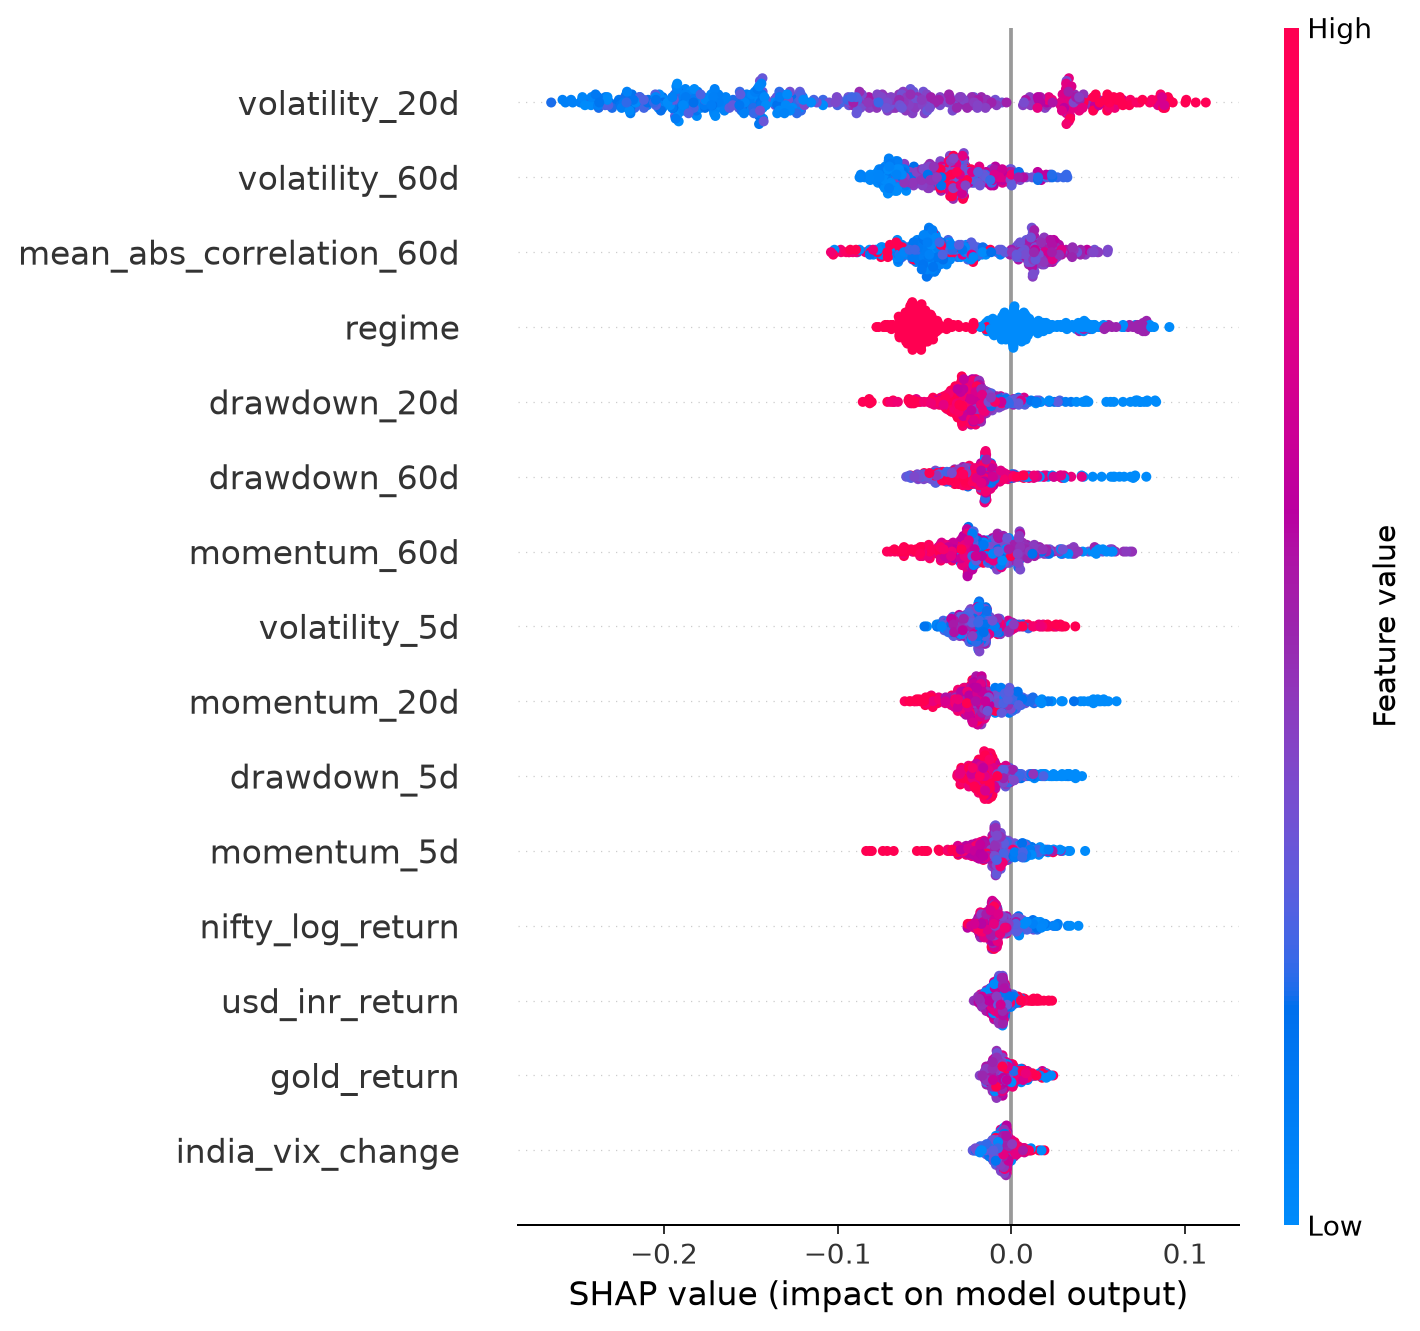
\includegraphics[width=0.92\textwidth]{figures/shap_feature_summary.png}
\caption{SHAP feature summary for the full NIFTY-Sentinel model. The plot explains which features most strongly influence the stress classifier across the evaluated sample.}
\label{fig:shap}
\end{figure}

The final dashboard export identifies volatility, drawdown, regime, and connectedness features among the leading model drivers. This is consistent with the research design: stress should be explained by market instability, loss depth, changing regimes, and cross-asset synchronization rather than by price level alone.

\section{Dashboard Implementation}

The dashboard is implemented in Streamlit and also exported as a static GitHub Pages version. The dashboard contains the following sections:

\begin{itemize}
    \item executive monitor with stress probability, warning level, NIFTY close, regime, and connectedness;
    \item market layers with volatility, drawdown, return, momentum, and connectedness charts;
    \item risk appetite view using India VIX, USD/INR, and gold proxies;
    \item connectedness heatmap and strongest cross-asset correlation links;
    \item model explainability using feature-importance and warning-band diagnostics;
    \item historical case studies for 2013, 2018, 2020, and 2022;
    \item methodology notes and data warnings.
\end{itemize}

The dashboard is important because the project is not only a modelling exercise. The final output must communicate model behavior to a user who needs to understand why the warning level changed. For that reason, the dashboard avoids presenting the probability as a trading recommendation. It frames the output as decision support for academic and risk-monitoring use.

\section{Discussion}

The results support three main observations. First, financial stress is multidimensional. Volatility, drawdown, connectedness, and regime state all provide information that is not captured by price level alone. Second, nonlinear models can improve stress classification, but the gain is not large enough to justify ignoring interpretability. Third, ablation analysis is essential because every additional feature layer should earn its place in the system.

The strongest practical value of NIFTY-Sentinel is its end-to-end structure. A user can trace the system from raw data to engineered features, from features to regimes and connectedness, from model outputs to warning bands, and from warning bands to dashboard explanations. This transparency is especially important for financial machine learning projects because unverified models can easily produce misleading confidence.

\section{Limitations}

The project has several limitations.

\begin{enumerate}
    \item The current project uses actual historical public-market data, but it has not yet been fully cross-validated against official NSE and RBI archives.
    \item The stress label is a modelling construct and should be tested against alternative definitions.
    \item Thresholds for warning levels are simple and require calibration for real institutional use.
    \item The model uses historical market proxies and does not include macroeconomic announcements, liquidity microstructure, news sentiment, or option-implied distribution measures beyond volatility proxies.
    \item The results are based on historical validation and do not prove causal relationships.
\end{enumerate}

These limitations should be addressed before presenting the system as a final operational risk model. For the current academic project stage, they are acceptable as long as they are explicitly disclosed.

\section{Future Work}

Several extensions would strengthen the project.

\begin{itemize}
    \item Cross-validate the public-market dataset against official NSE and RBI data and rerun all notebooks.
    \item Add Bank NIFTY, sectoral indices, bond yields, and volume-based liquidity features.
    \item Calibrate warning thresholds using cost-sensitive evaluation.
    \item Add probability calibration methods such as isotonic regression or Platt scaling.
    \item Compare Random Forest with XGBoost, LightGBM, and temporal neural models.
    \item Add automated dashboard refresh and model monitoring.
    \item Expand case studies with detailed event windows around 2013 taper stress, 2018 IL\&FS stress, 2020 COVID-19, and 2022 inflation tightening.
\end{itemize}

\section{Conclusion}

NIFTY-Sentinel demonstrates a complete explainable machine learning workflow for Indian equity market stress monitoring. The system combines interpretable financial features, latent regime detection, connectedness measurement, supervised classification, ablation analysis, explanation plots, and dashboard deployment. The prototype results show that the full layered model improves on a market-only baseline and produces a usable stress probability timeline. More importantly, the project establishes a disciplined research structure that avoids treating machine learning as a black box.

The system should be understood as an early-warning intelligence dashboard rather than a trading model. Its value lies in combining multiple signals into an interpretable probability and making the evidence visible through charts. With official data integration and further validation, the framework can become a strong academic demonstration of explainable financial stress modelling for the Indian market.

\begin{thebibliography}{99}

\bibitem[Al-Awadhi et al.(2020)]{alawadhi2020covid}
Al-Awadhi, A. M., Alsaifi, K., Al-Awadhi, A., and Alhammadi, S. (2020). Death and contagious infectious diseases: Impact of the COVID-19 virus on stock market returns. \textit{Journal of Behavioral and Experimental Finance}, 27, 100326.

\bibitem[An et al.(2022)]{genberg2022banking}
An, Z., Genberg, H., and Yu, X. (2022). A machine learning approach to rank the determinants of banking crises over time and across countries. \textit{Journal of International Money and Finance}, 129, 102739.

\bibitem[Dua and Tuteja(2021)]{dua2021regime}
Dua, P., and Tuteja, D. (2021). Regime shifts in the behaviour of international currency and equity markets: A Markov-switching analysis. \textit{Journal of Quantitative Economics}, 19(Suppl. 1), 309--336.

\bibitem[Duprey and Klaus(2022)]{duprey2022early}
Duprey, T., and Klaus, B. (2022). Early warning or too late? A (pseudo-)real-time identification of leading indicators of financial stress. \textit{Journal of Banking \& Finance}, 138, 106196.

\bibitem[Fons et al.(2020)]{fons2020hmm}
Fons, E., Dawson, P., Yau, J., Zeng, X.-J., and Keane, J. (2020). A novel dynamic asset allocation system using Feature Saliency Hidden Markov models for smart beta investing. \textit{Expert Systems with Applications}, 163, 113720.

\bibitem[Giudici and Abu Hashish(2020)]{giudici2020hmm}
Giudici, P., and Abu Hashish, I. (2020). A hidden Markov model to detect regime changes in cryptoasset markets. \textit{Quality and Reliability Engineering International}, 36(6), 2057--2065.

\bibitem[Guru and Das(2021)]{guru2021covid}
Guru, B. K., and Das, A. (2021). COVID-19 and uncertainty spillovers in Indian stock market. \textit{MethodsX}, 8, 101199.

\bibitem[Ilesanmi and Tewari(2020)]{ilesanmi2020southafrica}
Ilesanmi, K. D., and Tewari, D. D. (2020). Financial stress index and economic activity in South Africa: New evidence. \textit{Economies}, 8(4), 110.

\bibitem[Jarmulska(2022)]{jarmulska2022rf}
Jarmulska, B. (2022). Random forest versus logit models: Which offers better early warning of fiscal stress? \textit{Journal of Forecasting}, 41(4), 803--826.

\bibitem[Li(2021)]{li2021asymmetric}
Li, W. (2021). COVID-19 and asymmetric volatility spillovers across global stock markets. \textit{The North American Journal of Economics and Finance}, 58, 101474.

\bibitem[Naeem et al.(2021)]{naeem2021covid}
Naeem, M. A., Sehrish, S., and Costa, M. D. (2021). COVID-19 pandemic and connectedness across financial markets. \textit{Pacific Accounting Review}, 33(2), 165--178.

\bibitem[Pang et al.(2021)]{panga2021oilfsi}
Pang, D., Ma, F., Wahab, M. I. M., and Zhu, B. (2021). Financial stress and oil market volatility: New evidence. \textit{Applied Economics Letters}. Published online 24 August 2021.

\bibitem[Rao et al.(2021)]{rao2021vulnerability}
Rao, P., Goyal, N., Kumar, S., Hassan, M. K., and Shahimi, S. (2021). Vulnerability of financial markets in India: The contagious effect of COVID-19. \textit{Research in International Business and Finance}, 58, 101462.

\bibitem[Sahoo(2021)]{sahoo2021indiafsi}
Sahoo, J. (2021). Financial stress index, growth and price stability in India: Some recent evidence. \textit{Transnational Corporations Review}, 13(2), 222--236.

\bibitem[Sahoo and Kumar(2023)]{sahoo2023sectoral}
Sahoo, S., and Kumar, S. (2023). Volatility spillover among the sectoral indices of the Indian capital market: Evidence from the COVID period. \textit{Indian Journal of Finance}, 17(9).

\bibitem[Samitas et al.(2020)]{samitas2020ml}
Samitas, A., Kampouris, E., and Kenourgios, D. (2020). Machine learning as an early warning system to predict financial crisis. \textit{International Review of Financial Analysis}, 71, 101507.

\bibitem[Tang et al.(2024)]{tang2024systemic}
Tang, P., Tang, T., and Lu, C. (2024). Predicting systemic financial risk with interpretable machine learning. \textit{The North American Journal of Economics and Finance}, 71, 102088.

\bibitem[Adekoya and Oliyide(2021)]{adekoya2021covidconnected}
Adekoya, O. B., and Oliyide, J. A. (2021). How COVID-19 drives connectedness among commodity and financial markets: Evidence from TVP-VAR and causality-in-quantiles techniques. \textit{Resources Policy}, 70, 101898.

\bibitem[Wang et al.(2021)]{sectoral2022us}
Wang, Z., Yao, C., and Li, X. (2022). Sectoral connectedness: New evidence from US stock market during COVID-19 pandemics. \textit{Finance Research Letters}, 45, 102124.

\bibitem[Tang et al.(2022)]{survey2022fts}
Tang, Y., Song, Z., Zhu, Y., Yuan, H., Hou, M., Ji, J., Tang, C., and Li, J. (2022). A survey on machine learning models for financial time series forecasting. \textit{Neurocomputing}, 512, 363--380.

\bibitem[Zhang and Hamori(2021)]{zhang2021oilstock}
Zhang, W., and Hamori, S. (2021). Crude oil market and stock markets during the COVID-19 pandemic: Evidence from the US, Japan, and Germany. \textit{International Review of Financial Analysis}, 74, 101702.

\bibitem[Zhang et al.(2022)]{zhang2022xai}
Zhang, Z., Wu, C., Qu, S., and Chen, X. (2022). An explainable artificial intelligence approach for financial distress prediction. \textit{Information Processing \& Management}, 59(4), 102988.

\bibitem[Zhang et al.(2023)]{asoc2023xai}
Zhang, Y., Li, X., and Guo, S. (2023). Extending machine learning prediction capabilities by explainable AI in financial time series prediction. \textit{Applied Soft Computing}, 132, 109876.

\bibitem[Lu et al.(2023)]{eap2023indiaCommodity}
Lu, R., Xu, W., Zeng, H., and Zhou, X. (2023). Volatility connectedness among the Indian equity and major commodity markets under the COVID-19 scenario. \textit{Economic Analysis and Policy}, 78, 1465--1481.

\bibitem[Maharana et al.(2024)]{jrfm2024indiaSpillover}
Maharana, N., Panigrahi, A. K., and Chaudhury, S. K. (2024). Volatility persistence and spillover effects of Indian market in the global economy: A pre- and post-pandemic analysis using VAR-BEKK-GARCH model. \textit{Journal of Risk and Financial Management}, 17(7), 294.

\bibitem[Ghosh and Sanyal(2021)]{marketfear2021india}
Ghosh, I., and Sanyal, M. K. (2021). Introspecting predictability of market fear in Indian context during COVID-19 pandemic: An integrated approach of applied predictive modelling and explainable AI. \textit{International Journal of Information Management Data Insights}, 1(2), 100039.

\bibitem[Mundra and Bicchal(2020)]{jfep2020indiafsi}
Mundra, S., and Bicchal, M. (2020). Evaluating financial stress indicators: Evidence from Indian data. \textit{Journal of Financial Economic Policy}, 13(1), 116--135.

\bibitem[Breiman(2001)]{breiman2001}
Breiman, L. (2001). Random forests. \textit{Machine Learning}, 45, 5--32.

\bibitem[Hamilton(1989)]{hamilton1989}
Hamilton, J. D. (1989). A new approach to the economic analysis of nonstationary time series and the business cycle. \textit{Econometrica}, 57(2), 357--384.

\bibitem[Lundberg and Lee(2017)]{lundberg2017}
Lundberg, S. M., and Lee, S. I. (2017). A unified approach to interpreting model predictions. \textit{Advances in Neural Information Processing Systems}.

\bibitem[Pedregosa et al.(2011)]{pedregosa2011}
Pedregosa, F., Varoquaux, G., Gramfort, A., Michel, V., Thirion, B., Grisel, O., Blondel, M., Prettenhofer, P., Weiss, R., Dubourg, V., Vanderplas, J., Passos, A., Cournapeau, D., Brucher, M., Perrot, M., and Duchesnay, E. (2011). Scikit-learn: Machine learning in Python. \textit{Journal of Machine Learning Research}, 12, 2825--2830.

\bibitem[Schwert(1989)]{schwert1989}
Schwert, G. W. (1989). Why does stock market volatility change over time? \textit{Journal of Finance}, 44(5), 1115--1153.

\bibitem[Tapkire and Arun(2023)]{tapkire2023food}
Tapkire, M. D., and Arun, V. (2023). Application of artificial intelligence to correlate food formulations to disease risk prediction: A comprehensive review. \textit{Journal of Food Science and Technology}, 60(9), 2350--2357. doi:10.1007/s13197-022-05550-w.

\bibitem[Arun et al.(2024)]{arun2024road}
Arun, V., Shashikala, B. M., Vani, H. Y., Tapkire, M., Anusuya, M. A., and Lavanya, M. S. (2024). Object detection using TensorFlow for road navigation: Enhancing safety for the visually impaired. In \textit{International Conference Summit on Artificial Intelligence}, 209--220. Springer. doi:10.1007/978-981-97-7592-7\_17.

\bibitem[Lavanya et al.(2024a)]{lavanya2024emotion}
Lavanya, M. S., Arun, V., Tapkire, M., and Suhaas, K. P. (2024). Transfer learning based facial emotion recognition. \textit{SN Computer Science}, 6(1), 35. doi:10.1007/s42979-024-03523-8.

\bibitem[Shashidhar et al.(2025)]{shashidhar2025heart}
Shashidhar, R., Vasishta, P., Hegde, A., Madhura, J., Roopa, M., and Tapkire, M. D. (2025). Early detection of heart blockages: The power of AI and feedforward neural networks. In \textit{2025 International Conference on Electronics, Computing, Communication and Control Technology}, 1--6. IEEE. doi:10.1109/ICECCC65144.2025.11064297.

\bibitem[Tapkire et al.(2025)]{tapkire2025gluten}
Tapkire, M., Arun, V., Lavanya, M. S., and Shashidhar, R. (2025). Gluten identification from food images using advanced deep learning and transfer learning methods. \textit{Journal of Food Science and Technology}, 62(6), 1164--1172. doi:10.1007/s13197-024-06158-y.

\bibitem[Manjunath et al.(2025)]{manjunath2025skin}
Manjunath, A. S., Shashidhar, R., Shashank, M. P., Tapkire, M., Roopa, M., and Kruthika, S. (2025). Advancing dermatological AI: A unified deep learning pipeline for skin lesion analysis. In \textit{2025 2nd Asia Pacific Conference on Innovation in Technology}, 1--7. IEEE. doi:10.1109/APCIT65661.2025.11410765.

\bibitem[Natesh et al.(2025)]{natesh2025diabetes}
Natesh, M., Ranjan Kumar, H. S., Vinutha, K., Tapkire, M., Sulthana, S., Swetha, K. R., and Bharath, K. N. (2025). Improved diabetes detection through integration of external risk factors and machine learning techniques. \textit{SN Computer Science}, 6(8), 1--18. doi:10.1007/s42979-025-04486-0.

\bibitem[Lavanya et al.(2024b)]{lavanya2024facialreview}
Lavanya, M. S., Arun, V., Tapkire, M., and Shichkina, Y. (2024). A review on facial expression recognition approaches, datasets and technologies. In \textit{International Conference on Intelligent Systems}, 53--68. Springer Nature Switzerland. doi:10.1007/978-3-032-04764-9\_5.

\bibitem[Shwetha et al.(2026)]{shwetha2026plant}
Shwetha, K. S., Ramji, B. R., Ujwal, U. J., Tapkire, M., Magi, S. M., and Madalgi, J. (2026). Deep learning applications in automated detection of plant diseases across diverse crops. \textit{Journal of Integrated Science and Technology}, 14(4), 1553. doi:10.62110/sciencein.jist.2026.v14.1553.

\bibitem[Arpitha et al.(2025)]{arpitha2025health}
Arpitha, T., Shashidhar, R., Pruthvi, C. N., Tapkire, M., and Meghana, J. (2025). A PSO-fuzzy approximate reasoning model for decision support in remote health monitoring. In \textit{International Conference on Soft Computing and its Engineering Applications}, 382--394. Springer Nature Switzerland. doi:10.1063/5.0331506.

\bibitem[Vinesh et al.(2026)]{vinesh2026mci}
Vinesh, T., Lavanya, M. S., Arun, V., Juremi, J., Tapkire, M., Shashikala, B. M., and Fatin, A. M. S. (2026). AI-powered assessments for mild cognitive impairment detection: A comprehensive review. In \textit{AIP Conference Proceedings}, 3440(1), 020038. AIP Publishing. doi:10.1063/5.0331506.

\bibitem[Lavanya et al.(2026)]{lavanya2026mcipred}
Lavanya, M. S., Arun, V., Tapkire, M., Vanamala, C. K., Padma, M. T., Naganna, M., and Prakash, V. (2026). Hybrid optimization-based machine learning framework for predicting mild cognitive impairment progression. \textit{International Journal of Computer Information Systems and Industrial Management Applications}, 18(2), 203--214.

\end{thebibliography}

\end{document}

